\documentclass[conference]{IEEEtran}
%\IEEEoverridecommandlockouts
% The preceding line is only needed to identify funding in the first footnote. If that is unneeded, please comment it out.
\usepackage{cite}
\usepackage{amsmath,amssymb,amsfonts,mathtools}
\usepackage{algorithmic}
\usepackage{graphicx}
\usepackage{textcomp}
\usepackage{xcolor}
%\usepackage[numbers,sort&compress]{natbib}
\usepackage{hyperref}

\def\BibTeX{{\rm B\kern-.05em{\sc i\kern-.025em b}\kern-.08em
    T\kern-.1667em\lower.7ex\hbox{E}\kern-.125emX}}
\renewcommand{\IEEEQED}{\IEEEQEDopen}

\newtheorem{theorem}{Theorem}
\newtheorem{lemma}{Lemma}
\newtheorem{proposition}{Proposition}
\newtheorem{corollary}{Corollary}
\begin{document}

\title{Connectivity of Shadowing-Enhanced Device-to-Device Networks on Poisson-Voronoi Street Systems
%\thanks{Identify applicable funding agency here. If none, delete this.}
}

\author{\IEEEauthorblockN{Quentin Le Gall\IEEEauthorrefmark{1}, Elie Cali\IEEEauthorrefmark{1}, Taoufik En-Najjary\IEEEauthorrefmark{1} and Bart\l{}omiej B\l{}aszczyszyn\IEEEauthorrefmark{2}}
\IEEEauthorblockA{\IEEEauthorrefmark{1}Modelling and Statistical Analysis, Orange Labs Networks, Ch\^{a}tillon, France\\
Email: quentin1.legall@orange.com, elie.cali@orange.com and taoufik.ennajjary@orange.com}
\IEEEauthorblockA{\IEEEauthorrefmark{2}Dynamics of Geometric Networks, Inria-ENS, Paris, France\\
Email: bartek.blaszczyszyn@ens.fr}}

\maketitle

\begin{abstract}
This is the abstract. It will be typed later.
\end{abstract}

\begin{IEEEkeywords}
Device-to-device networks, connectivity, shadowing, continuum percolation
\end{IEEEkeywords}

\section{Introduction and Motivations}
Introduction will be typed later. 

\section{Network Model}
\subsection{Description of the model}
%What shall I define? percolation? connected component? PVT? How far can I assume the reader knows?
The network model relies on three major elements: the street model, the respective distributions of users and relays and the device-to-device (D2D) connectivity mechanism. \\
\indent First, following \cite{courtat_promenade_2012,chiu_stochastic_2013}, we model the street system by a planar Poisson-Voronoi tessellation (PVT) generated by a homogeneous Poisson Point process (PPP) in $\mathbb{R}^{2}$ of intensity $\lambda_{S} > 0$. In particular, $S$ is stationary, stabilising and asymptotically essentially connected, as presented in \cite{hirsch_continuum_2017}. We denote by $V$ (respectively $E$) the set of vertices (respectively edges) of $S$. Letting $\nu_{1}(T \cap B)$ measuring the total edge length of $S$ in any observation window defined by a Borel set $B$, we  denote by $\gamma \coloneqq \mathbb{E}\left[\nu_{1}\left(S \cap \left[-1/2;1/2\right]^{2}\right)\right]$ the total street length per unit area, expressed in km/km\textsuperscript{2}. It is a well-known fact \cite{moller_random_1989,moller_lectures_2012} that $\gamma = 2\sqrt{\lambda_{S}}$ when $S$ is a PVT. Typical values are $\gamma \approx 20 \: \text{km/km}^{2}$ for a city center of a classical European major city, while $\gamma = 1  \: \text{km/km}^{2}$ for rural areas. Since $\gamma$ is an intrinsic characteristic determined by geographical location, we will consider it to be a fixed parameter of the problem modelled here.  \\ %Talk about typical values? 
\indent Users are equipped with mobile devices and distributed according to a Cox point process $X$ driven by the random intensity measure $\lambda \nu_{1}(S \cap dx)$, where $\lambda \geq 0$ is the user intensity expressed in km\textsuperscript{-1} (the case $\lambda = 0$ corresponds to an absence of users and a D2D network only relying on relays placed by operators). Equivalently, whenever $\lambda > 0$, this means that conditioned on any realisation $S$ of the street system, $X$ is a Poisson point process with mean measure $\lambda \nu_{1}(S \cap dx)$. In particular, for any street segment $e \in E$, the number of users lying on $e$ is a Poisson random variable with parameter $\lambda \nu_{1}(e)$ and all users are spread independently and uniformly on $e$. In addition, for any two distinct street segments $e \neq e'$, the number of users lying on $e$ and the number of users lying on $e'$ are independent random variables.\\
\indent Network relays are spread on the crossroads of the street system according to a Bernoulli point process $Y$ of parameter $p \in \left[0,1\right]$. In other words, for each $v \in V$, a relay is placed at $v$ with probability $p$, independently from the state of any other crossroad in $V \setminus \lbrace v\rbrace$. \\
\indent Finally, assuming a constant communication radius $r >0$ (expressed in kilometers) as in \cite{glauche_continuum_2003}, and letting $Z \coloneqq X \cup Y$ denote the superposition of the users and the relays point processes, two distinct network agents (either relays of users devices) are connected by a device-to-device (D2D) link if and only if they are in line of sight (LOS) and of reciprocal Euclidean distance smaller than $r$, i.e. :
\begin{equation}
\label{connectivity_mechanism}
\forall \, i \neq j, \: Z_{i} \leftrightsquigarrow Z_{j} \Leftrightarrow 
\left\{
\begin{array}{l}
\exists \, e \in E, \, Z_{i} \in E  \  \text{and} \  Z_{j} \in E \\
\lVert Z_{i} - Z_{j} \rVert \leq r
\end{array}
\right.
\end{equation}
\indent The network is then represented by the connectivity graph $\mathcal{G}_{r,\lambda,p}$ whose vertices are the points of $Z$ and where an undirected edge $\lbrace Z_{i},Z_{j}\rbrace, \, i \neq j $ is drawn if and only if $Z_{i} \leftrightsquigarrow Z_{j}$. Connectivity of the network consisting in the possibility of establishing long-range communications, we are thus interested in assessing whether there exists an infinite connected component of the connectivity graph for a given set of parameters $(r,\lambda,p)$. In other words, we are driven to seek whether the connectivity graph percolates \cite{meester_continuum_1996} or not. 
\subsection{Main assumptions related to the model}
\label{assumption}
The former description of the model implies several assumptions, which we justify here. \\
\indent Note first that we model the street system as a two-dimensional tessellation, hence considering the problem to be planar. Indeed, we chose not to consider reflexions of the waves in a first step, for the sake of simplicity. As for diffractions, they are negligible in front of direct radio propagation on a given street. Indeed, consider the simplest case of non-line-of-sight (NLOS) propagation of a radio signal with frequency $f$ between a source and a target separated by only one building, of height $h$ and width $w$. Denote by $r_{1}$ (respectively $r_{2}$) the distance between the source (respectively the target) and the building. Then, using Bullington's method \cite{bullington1947radio}, the loss due to knife-edge diffraction by the two upper corners of the building can be approximated with the following formula: %shall I enter into so much detail? %compute a typical value? %names of the quantities involved?
\begin{equation}
\label{fading}
L_{d} \coloneqq 20\log_{10}\vert F \vert \: ,
\end{equation}
where $F$ is the complex Fresnel integral defined by the following equations:
\begin{equation}
\label{fresnel-integral}
F \coloneqq \frac{1+j}{2} \int_{\nu}^{+\infty} e^{-j\pi t^{2}/2}dt
\end{equation}
\begin{equation}
\label{lasteq}
\nu = -h\left(1+\frac{w}{r_{1}+r_{2}}\right)\sqrt{\frac{2f}{c}\left(\frac{1}{r_{1}}+\frac{1}{r_{2}}\right)} \quad ,
\end{equation}
where $j$ denotes the complex imaginary unit ($j^{2}=-1$) in \eqref{fresnel-integral}, while $c$ denotes, in \eqref{lasteq}, the velocity of the wave in the considered medium. A short computation with typical values encountered for a D2D network in an urban environment leads to a sufficiently high loss in comparison with direct propagation pathloss. Since in reality, multiple diffractions occur on the edges of one or several buildings separating a source and a target being in NLOS, we can indeed assume that diffractions can be neglected in front of LOS direct radio propagation. \\
\indent As in \cite{glauche_continuum_2003}, we assume a constant communication radius for the sake of simplicity. This also implies that we assume the transmission power of all devices and network relays to be constant. \\
\indent The connectivity mechanism defined by \eqref{connectivity_mechanism} only allows for LOS communications between a source and a target (whether they are a relay of an actual user equipped with a device). Equivalently, we consider that the physical obstacles encountered in our model are sufficiently absorbing to let any signal being transmitted through them.  Hence, our model somehow features a perfect shadowing situation, which is the main novelty of our work. \\
\indent Finally, we also neglect any interference phenomenon or user mobility for the sake of simplicity, which is of course far from reality in the context of D2D networks. 
\subsection{Simulation method}
All of our numerical experiments have been performed using the statistical software R \cite{team2014r}. For time-constraints reasons, we cannot simulate an infinite graph and hence choose a squared simulation window of side $win$, expressed in kilometers. When possible, $win = 30 \: \text{km}$ is chosen so as to avoid boundary effects. Contrary to \cite{cali2018percolation,mertens_continuum_2012}, we chose not to simulate on a torus-traced window: this is mainly for the sake of simplicity, as we had to deal with a practical and time-saving way to label network agents on streets to only allow for LOS connections. We are very much aware of this simplification and this could be a source of amelioration for future work. Nevertheless, taking a sufficiently large simulation window already provides interesting and exploitable results.\\
\indent For a set of parameters $(r,\lambda,p)$, we first simulate a PVT $S$ with the desired parameter $\gamma$. Then, we label each street segment with a unique number. Thereafter, we simulate the users' Cox point process and the relays' Bernoulli process. Each user is lying on a unique street, while each relay is located on a crossroad at the intersection of several streets (3 in average, see \cite{okabe_spatial_1992,chiu_stochastic_2013,blaszczyszyn_stochastic_2018}). We assign to each user (respectively each relay) the label of the unique street (respectively the label of the streets) it is located on. As a matter of fact, two network agents are in LOS if and only if they share a common label. Determining all existing connexions in an optimized way is thereafter straightforward: arrange the simulated network agents by street segment label, only keep the street segments containing at least two distinct network agents and then, for each street segment, compute the successive distances from one agent to the next one. If only one disconnection (i.e. two consecutive network agents separated by a gap larger than the communication threshold $r$) occurs on a given street segment, then it is not necessary to continue the computations for this street segment. We then keep track of the connected components of the simulated graph by using a union-find algorithm \cite{knuthart,sedgewick2011algorithms,newman2001fast}. Finally, we declare the graph percolates if there exists a left-right or a top-bottom crossing of the simulation window by a connected component. We then iterate this process and are thus able to compute the proportion of simulations where the graph $\mathcal{G}_{r,\lambda,p}$ percolates for a given set of parameters $(r,\lambda,p)$.  \\
\indent Similarly to \cite{cali2018percolation}, our model features scaling invariances: the Bernoulli process of relays is by definition motion-invariant \cite{blaszczyszyn_stochastic_2018}, while changing $\gamma$ to $a\gamma$ for $a>0$ is equivalent to zooming or unzooming to a rescaled simulation window where $\lambda$ has changed to $a\lambda$ and $r$ to $r/a$. Therefore, considering the two dimensionless parameters $\lambda / \gamma$ and $r\gamma$ for simulations is of great practical interest: it allows us to consider $\gamma$ as fixed for numerical as well as theoretical perspectives.  %is that so even with relays?

\subsection{Methodology}
All parameters of our model are correlated. However, it seems relevant to  consider the influence of the relay proportion $p$ as a starting point. Indeed, since our model only allows for LOS communications, the presence of a relay is necessary to hop from a given street to another, and hence relays seem to be critical to establish long-range communications. \\
\indent Another interesting parameter to be studied in its own is the communication radius $r$. Even if the probability of finding an edge of arbitrarily large length in a PVT is positive \cite{okabe_spatial_1992}, the maximum edge length in a bounded Borel set such as our simulation window is an almost surely bounded random variable \cite{chiu_stochastic_2013}. Therefore, choosing $r$ to be somehow sufficiently large should allow to bypass the need for user to establish long-range communications if the relays are present in a sufficiently large proportion $p$. \\
\indent Finally, the last question studied in this paper is on when users play a key role in the multihop D2D network simulated. In other words, what is the critical density \cite{meester_continuum_1996} $\lambda_{c} \coloneqq \lambda_{c}(r,p)$ ensuring percolation of the connectivity graph $\mathcal{G}_{r,\lambda,p}$ ?


\section{Influence of the relay proportion}
\label{relay-influence}
Studying the relay proportion $p$ in its own right seems relevant, as any infinite connected component of the connectivity graph $\mathcal{G}_{r,\lambda,p}$ contains an infinite number of relays. \\
\indent Our first theoretical result is a minimality condition on  $p$ for the possibility of percolation of the connectivity graph $\mathcal{G}_{r,\lambda,p}$. %open site or occupied site? closed site or vacant site?
To this end, we consider another percolation model: the Bernoulli site percolation model \cite{grimmett1999percolation} on $S$. In this model, each vertex of $S$ is either open (i.e. present) with probability $\tilde{p} \in \left[0,1\right]$ or closed (i.e. absent) with probability $1 - \tilde{p}$. Denote by $\tilde{\mathcal{G}}_{\tilde{p}}$ the subgraph of $S$ obtained by only keeping the open vertices of $S$ (i.e. $\lbrace v \in V: v \; \text{is open} \rbrace$) and the edges of $E$ connecting them. As usual, say that $\tilde{\mathcal{G}}_{\tilde{p}}$ percolates \cite{grimmett1999percolation, meester_continuum_1996} if it has an infinite connected component. Define as usual the percolation threshold:
\begin{equation}
\label{critical_site}
p_{c}^{\text{bond, PVT}} \coloneqq \inf \lbrace p \geq 0, \; \tilde{\mathcal{G}}_{\tilde{p}} \text{\: percolates} \rbrace
\end{equation}
A straightforward consequence of the stationarity of $S$ is that $p_{c}^{\text{bond, PVT}}$ is independent of the intensity $\lambda_{S}$ of the PPP having generated $S$. It is a well-known fact that $p_{c}^{\text{bond, PVT}}\in (0,1)$ \cite{grimmett1999percolation, ziesche2016bernoulli}. Moreover, \cite{neher2008topological} found the following theoretical estimate: $p_{c}^{\text{bond, PVT}} \approx 0.7151 $, while \cite{becker_percolation_2009}, using Monte-Carlo simulations with periodic boundary conditions, numerically determines $p_{c}^{\text{bond, PVT}} \approx 0.71410 \pm 0.00002$. We also performed Monte-Carlo simulations on our own to check whether we were able to obtain a sufficiently reasonable estimate of $p_{c}^{\text{bond,PVT}}$ and obtained the graph shown in Fig.\ref{site-threshold}: the green curve is the function $p \mapsto f(p)$, where $f(p)$ represents the number of times the simulated connectivity graph $\tilde{\mathcal{G}_{p}}$ percolates. A logistic model \begin{equation*}
\log\left(\frac{f(p)}{1-f(p)}\right)=ap+b
\end{equation*} 
given by the blue curve seems to fit a good approximation. Since the theoretical curve on an infinite tessellation would be a 0-1 curve with cutoff value $p_{c}^{\text{bond,PVT}}$ by ergodicity, we can reasonably use the approximation $f\left(p_{c}^{\text{bond,PVT}}\right) \approx 0.5$ to get the approximation
\begin{equation*}
p_{c}^{\text{bond,PVT}} \approx -\frac{b}{a} \; ,
\end{equation*}
where $a$ and $b$ are determined by linear regression. This led to the following estimate:
\begin{equation*}
p_{c}^{\text{bond,PVT}} \approx 0.71299 \;  %incertitude?
\end{equation*}
which is a fairly reasonable approximation for our purposes.
\begin{figure}[t!]
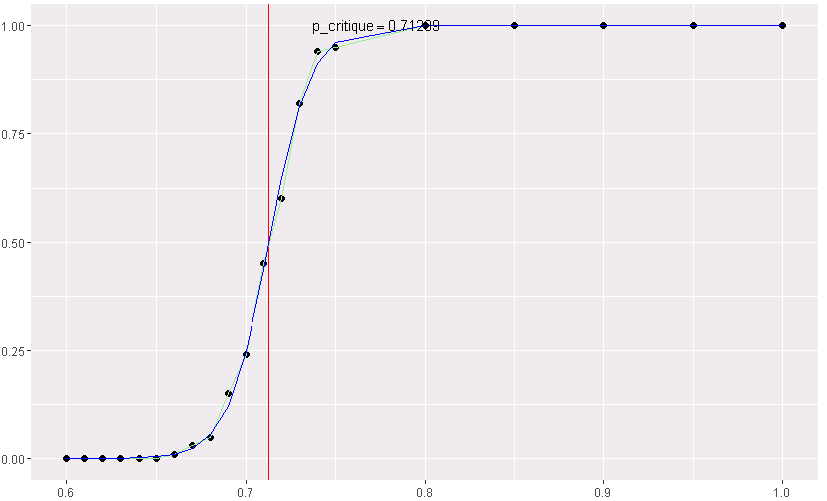
\includegraphics[width=\columnwidth]{Figures/PVT-site-threshold.png}
\caption{Estimation of the PVT site percolation threshold. The simulation window is of size 30x30 $\text{km}^{2}$ and the street linear intensity is $\gamma = 20 \; \text{km/km}^{2}$. The green curve is the simulated curve $p \mapsto f(p)$, the blue one is the logistic model and the red vertical line determines the intercept $p_{c}^{\text{bond,PVT}}$.}
\label{site-threshold}
\end{figure}\\

\indent On a theoretical perspective, by comparing percolation of the connectivity graph $\mathcal{G}_{r,\lambda,p}$ with Bernoulli site percolation on $S$, we obtained the following result: \\
\begin{theorem}[Minimality condition on $p$] \label{minimality_theorem} If $p<p_{c}^{\text{bond, PVT}}$, then, for all $r > 0$ and $\lambda \geq 0$, the graph $\mathcal{G}_{r,\lambda,p}$ does not percolate, i.e. long-distance multihop D2D communications are not possible.
\end{theorem}
\begin{IEEEproof} 
Let $p < p_{c}^{\text{bond, PVT}}$. Consider site percolation on $S$ with parameter $p$. Then, by \eqref{critical_site} the associated graph $\tilde{\mathcal{G}}_{p}$ does not percolate. But since $\mathcal{G}_{r,\lambda,p}$ is a subgraph of $\tilde{\mathcal{G}}_{p}$ for all $r \geq 0$ and $\lambda \geq 0$, the absence of percolation of $\tilde{\mathcal{G}}_{p}$ implies the absence of percolation of $\mathcal{G}_{r,\lambda,p}$. Hence the result.
\end{IEEEproof}
\vspace{\baselineskip}
\indent Theorem \ref{minimality_theorem} has the following practical consequence: an operator willing to rely on D2D to extend coverage via using a multihop D2D network must equip at least 71.5\% of the crossroads with relays or hotspots to counter shadowing effects. This represents a heavy investment, which needs to be counterbalanced. Only relying on users' devices to allow for long-distance connectivity is not a viable option. Finally, note that our result ensures a minimality condition on $p$ only. We were indeed able to find parameters such that even when $p=1$, i.e. all crossroads are equipped with relays, the connectivity graph does not percolate in the absence of users. A matching maximality result on $p$ is therefore unthinkable. 
%What else can I add here? What about my method and the p_site I found?

\section{Influence of the communication radius}
\label{radius-influence}
Another interesting parameter to be studied in its own is the communication radius $r$. Even though it is a physical constraint imposed by the type of D2D technology and link used \cite{asadi_survey_2014}, it is not unrealistic to think that the underlying geometry with the presence of a sufficiently high proportion could allow for long-range D2D communications even when the user density $\lambda$ is low. The mathematical intuition behind this is the following: in a PVT, there is a positive probability of finding an arbitrarily long edge, but our simulation windows (as well as real environments) are bounded, or consisting in several morphologically homogeneous bounded zones \cite{courtat_promenade_2012}. Therefore, the maximum edge length in a bounded observation window is a bounded random variable with high probability. Choosing a communication radius $r$ bigger than this former maximum and a sufficiently large proportion of relays $p$ should therefore lead to percolation of $\mathcal{G}_{r,0,p}$, and therefore for percolation of $\mathcal{G}_{r,\lambda,p}$ for any $\lambda \geq 0$, as adding users to the models can only enlarge the number of connexions, hence making percolation to occur easier. \\
\indent To this end, for several values of the parameter $\gamma$, we simulated a lot of PVTs on a window of size $win = 30 \; \text{km}$ and then stocked the length of all obtained edges in a list. This gave us a fairly good sample of the distribution of the length of the so-called typical edge \cite{muche2005poisson}, i.e. an edge of a PVT chosen at random. %better explain what the typical edge is
\begin{figure}[t!]
\centering
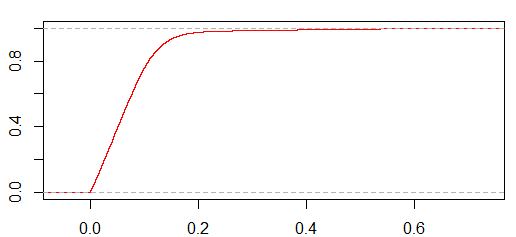
\includegraphics[width=\columnwidth]{Figures/PVT-street-length-20.png}
\caption{Empirical CDF of a PVT street system with $\gamma = 20 \; \text{km/km}^{2}$, i.e. an urban environment.}
\label{PVT-length-20}
\end{figure} 
We were then able to plot the empirical cumulative distribution functions (CDF) of the typical edge length. Fig \ref{PVT-length-20} shows an example of such a CDF in an urban environment. In that case, it is worth noticing that 90\% of the streets are shorter than 170 meters. \\
\indent For given $\gamma$ and $p$, the question of the possibility of percolation in the absence of users, (i.e. setting $\lambda =0$) is whether the critical radius $r_{0}$ is finite:
\begin{equation}
%can I write r0 = r0(p) to make implicit notation on dependence of p?
\label{critical-radius}
r_{0} = r_{0}(p) \coloneqq \inf \lbrace r > 0, \; \mathcal{G}_{r,0,p} \; \text{percolates} \rbrace < \infty
\end{equation}
\begin{figure}[t!]
\centering
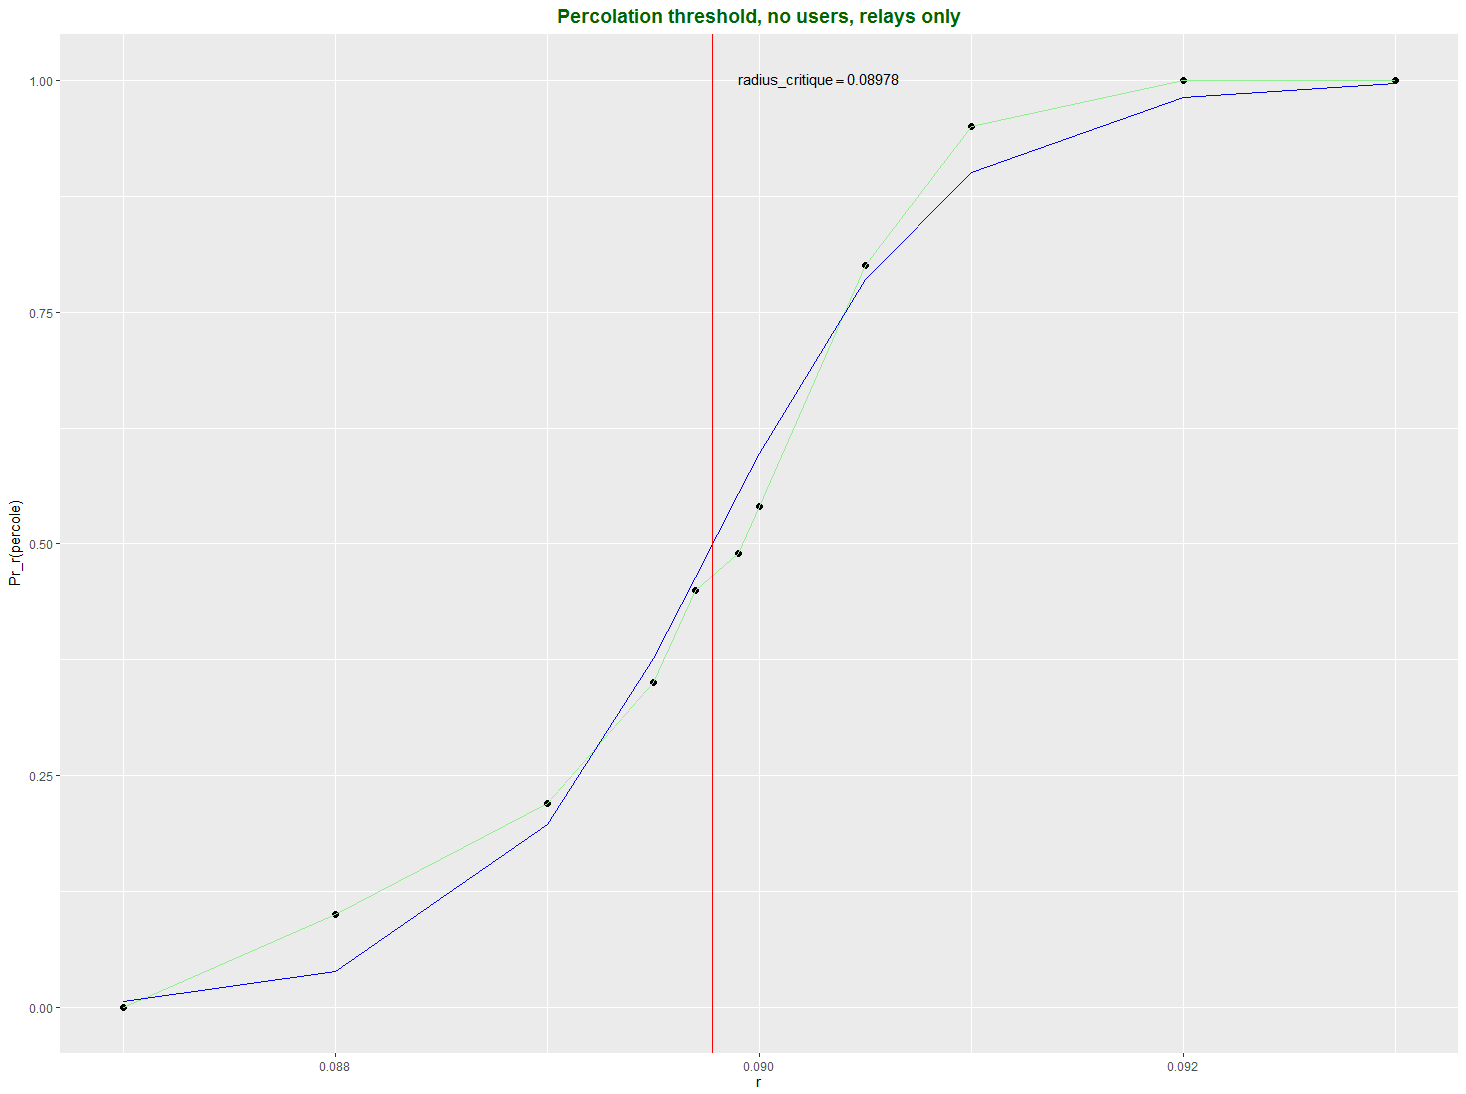
\includegraphics[width=\columnwidth]{Figures/sites-rgamma0-p_1.png}
\caption{Estimation of $r_{0}$ for $p=1$ and street linear intensity $\gamma = 20 \; \text{km/km}^{2}$. The simulation window is of size 30x30 $\text{km}^{2}$. The green curve is the simulated curve $r \mapsto g(r)$, the blue one is the logistic model and the red vertical line determines the intercept $r_{0}$.}
\label{good-logistic-rgamma0}
\end{figure}
\begin{figure}[t!]
\centering
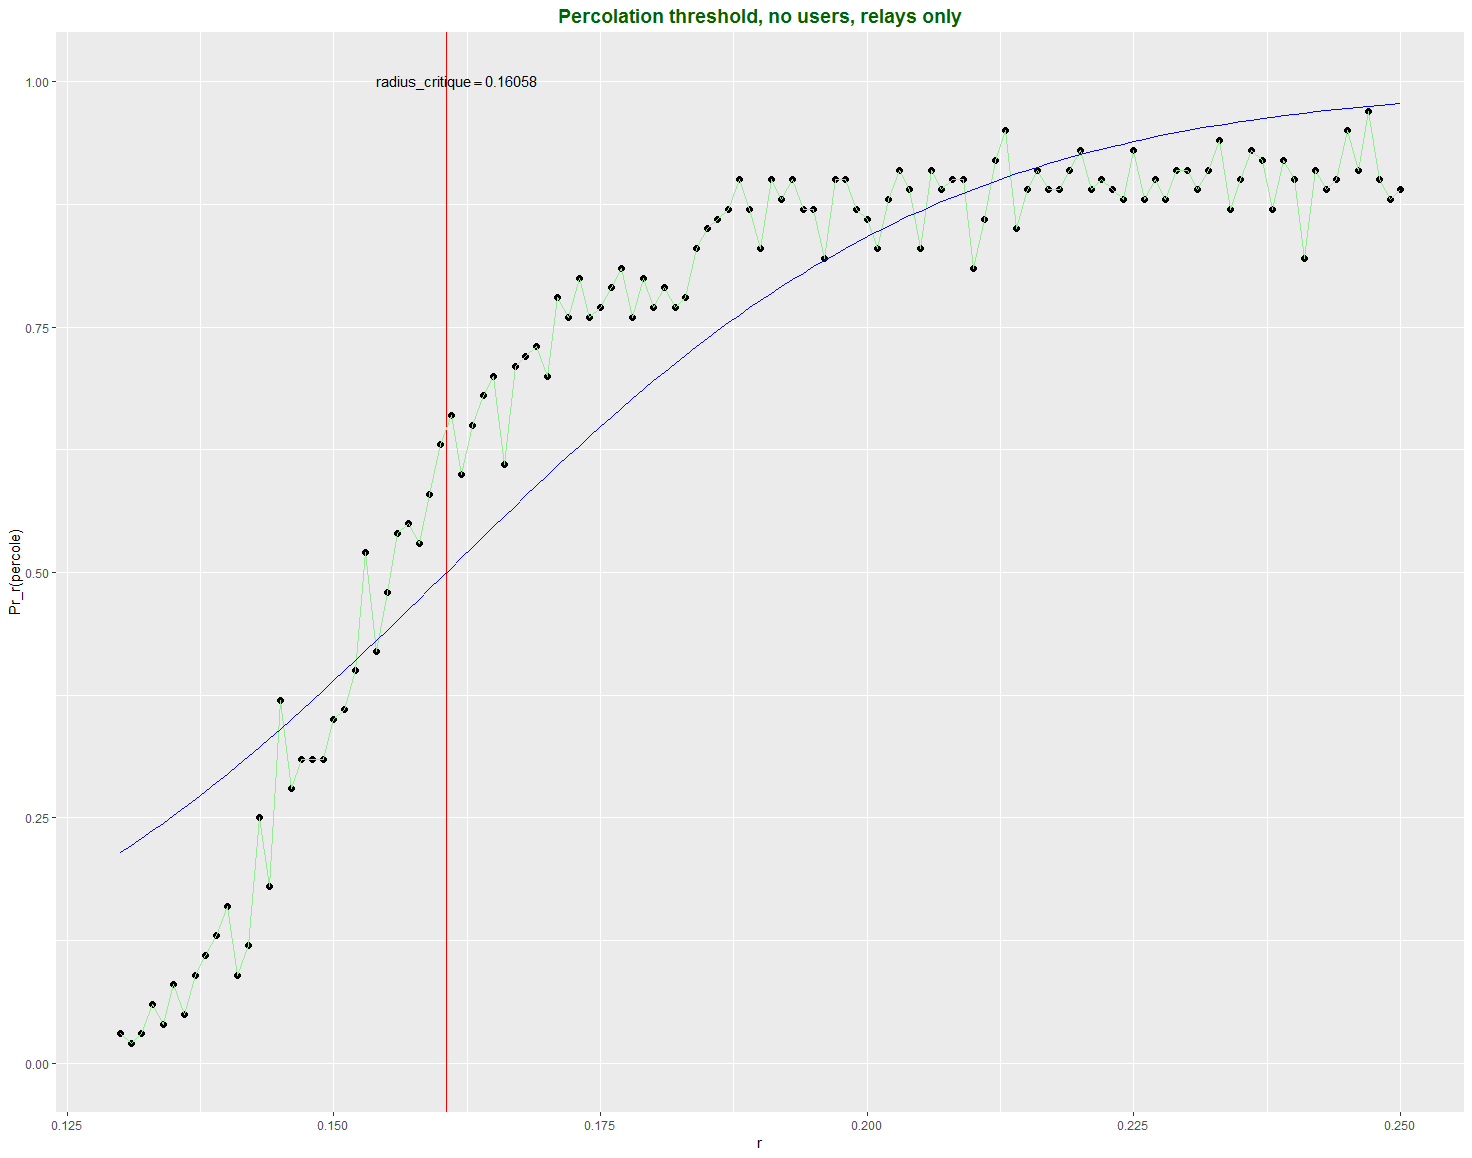
\includegraphics[width=\columnwidth]{Figures/sites-rgamma0-p_0_73.png}
\caption{Estimation of $r_{0}$ for $p=0.73$ and $\gamma = 20 \; \text{km/km}^{2}$. The simulation window is of size 30x30 $\text{km}^{2}$. The green curve is the simulated curve $r \mapsto g(r)$, the blue one is the logistic model and the red vertical line determines the intercept $r_{0}$. A logistic model does not yield a good fit of $g(r)$ anymore.}
\label{bad-logistic-rgamma0}
\end{figure} 
Therefore, we compute the proportion for a grid of values of $r$ the proportion $g(r)$ of simulations where the graph $\mathcal{G}_{r,0,p}$ percolates. Again, a logistic model yields a good fitting of the estimated curve, as long as $p$ is sufficiently far from the critical value $p_{c}^{\text{bond, PVT}}$. Finally, we estimate $r_{0}$ by the abscissa of the inflexion point of the logistic curve. Fig.\ref{good-logistic-rgamma0} illustrates an example when $p=1$. However, when $p$ approaches $p_{c}^{\text{bond, PVT}}$, the logistic model does not give a good fitting anymore, as can be seen in Fig.\ref{bad-logistic-rgamma0}. This can be explained by the following fact: when $p$ approaches $p_{c}^{\text{bond,PVT}}$, the relay proportion is not sufficient anymore to allow for site percolation on a large proportion of the simulated graphs (as shown in Fig.\ref{site-threshold}, the estimated percolation probability quickly decreases in the window $\left[0.72,0.74\right]$). By Theorem \ref{minimality_theorem}, if the graph $\tilde{\mathcal{G}}_{p}$ associated with the Bernoulli site percolation on $S$ does not percolate, then neither does $\mathcal{G}_{r,0,p}$. An additional explanation relies on the assumption (strongly believed to be true by analogy with the well-known Poisson Boolean model \cite{blaszczyszyn_stochastic_2018}) that the infinite connected component of $\mathcal{G}_{r,0,p}$ is almost surely unique. Therefore, for percolation of $\mathcal{G}_{r,0,p}$ to occur, the exact precise street segments belonging to the almost surely unique connected path crossing the simulation window have to let communications through, i.e. have relays present at their both endpoints. When $p$ approaches $p_{c}^{\text{bond,PVT}}$, the former becomes very unlikely.  \\
\indent The system started having an erratic behaviour around $p \approx 0.74$ and it then did not give any sense anymore to the estimation of $r_{0}$. Moreover, as stated in Section \ref{assumption}, the dimensionless parameter $r\gamma$ is scaling invariant. As a matter of fact, we present our results in Table \ref{tab-rgamma0} in terms of the parameter $r_{0}\gamma$. We also compute the corresponding critical radius $r_{0}$ in meters for an urban environment, i.e. setting $\gamma = 20 \; \text{km/km}^{2}$.
\begin{table}[t!]
\caption{Critical parameter $r_{0}\gamma$ and corresponding $r_{0}$ in an urban environment as a function of $p$}
\begin{center}
\begin{tabular}{|c|c|c|}
\hline
$p$ & $r_{0}\gamma$ & $r_{0}$ (meters), urban environment \\
\hline
0.75 & 2.8592 & 142.96  \\
0.76 & 2.7392 & 136.96 \\
0.77 & 2.6519 & 132.60 \\
0.78 & 2.559 & 127.95  \\
0.79 & 2.498 & 124.90 \\
0.80 & 2.4344 & 121.72  \\
0.85 & 2.1904 & 109.52 \\
0.90 & 2.035 & 101.75 \\
0.95 & 1.9006  & 95.03 \\
1 & 1.7956 & 89.78  \\
\hline
\end{tabular}
\label{tab-rgamma0}
\end{center}
\end{table}
\newline \indent As can easily be guessed, $r_{0}\gamma$ is decreasing with $p$. Moreover, it is worth noticing that, in an urban environment, which is easy to endow with relays, $r_{0}$ remains less than 150 meters, a technological threshold which, for one thing, does not seem physically unreachable \cite{lin_comprehensive_2013}, and which, on the other hand, was mentioned in \cite{asadi_survey_2014} for a significantly higher power efficiency of the network in comparison with a conventional cellular network. \\
\begin{figure}[t!]
\centering
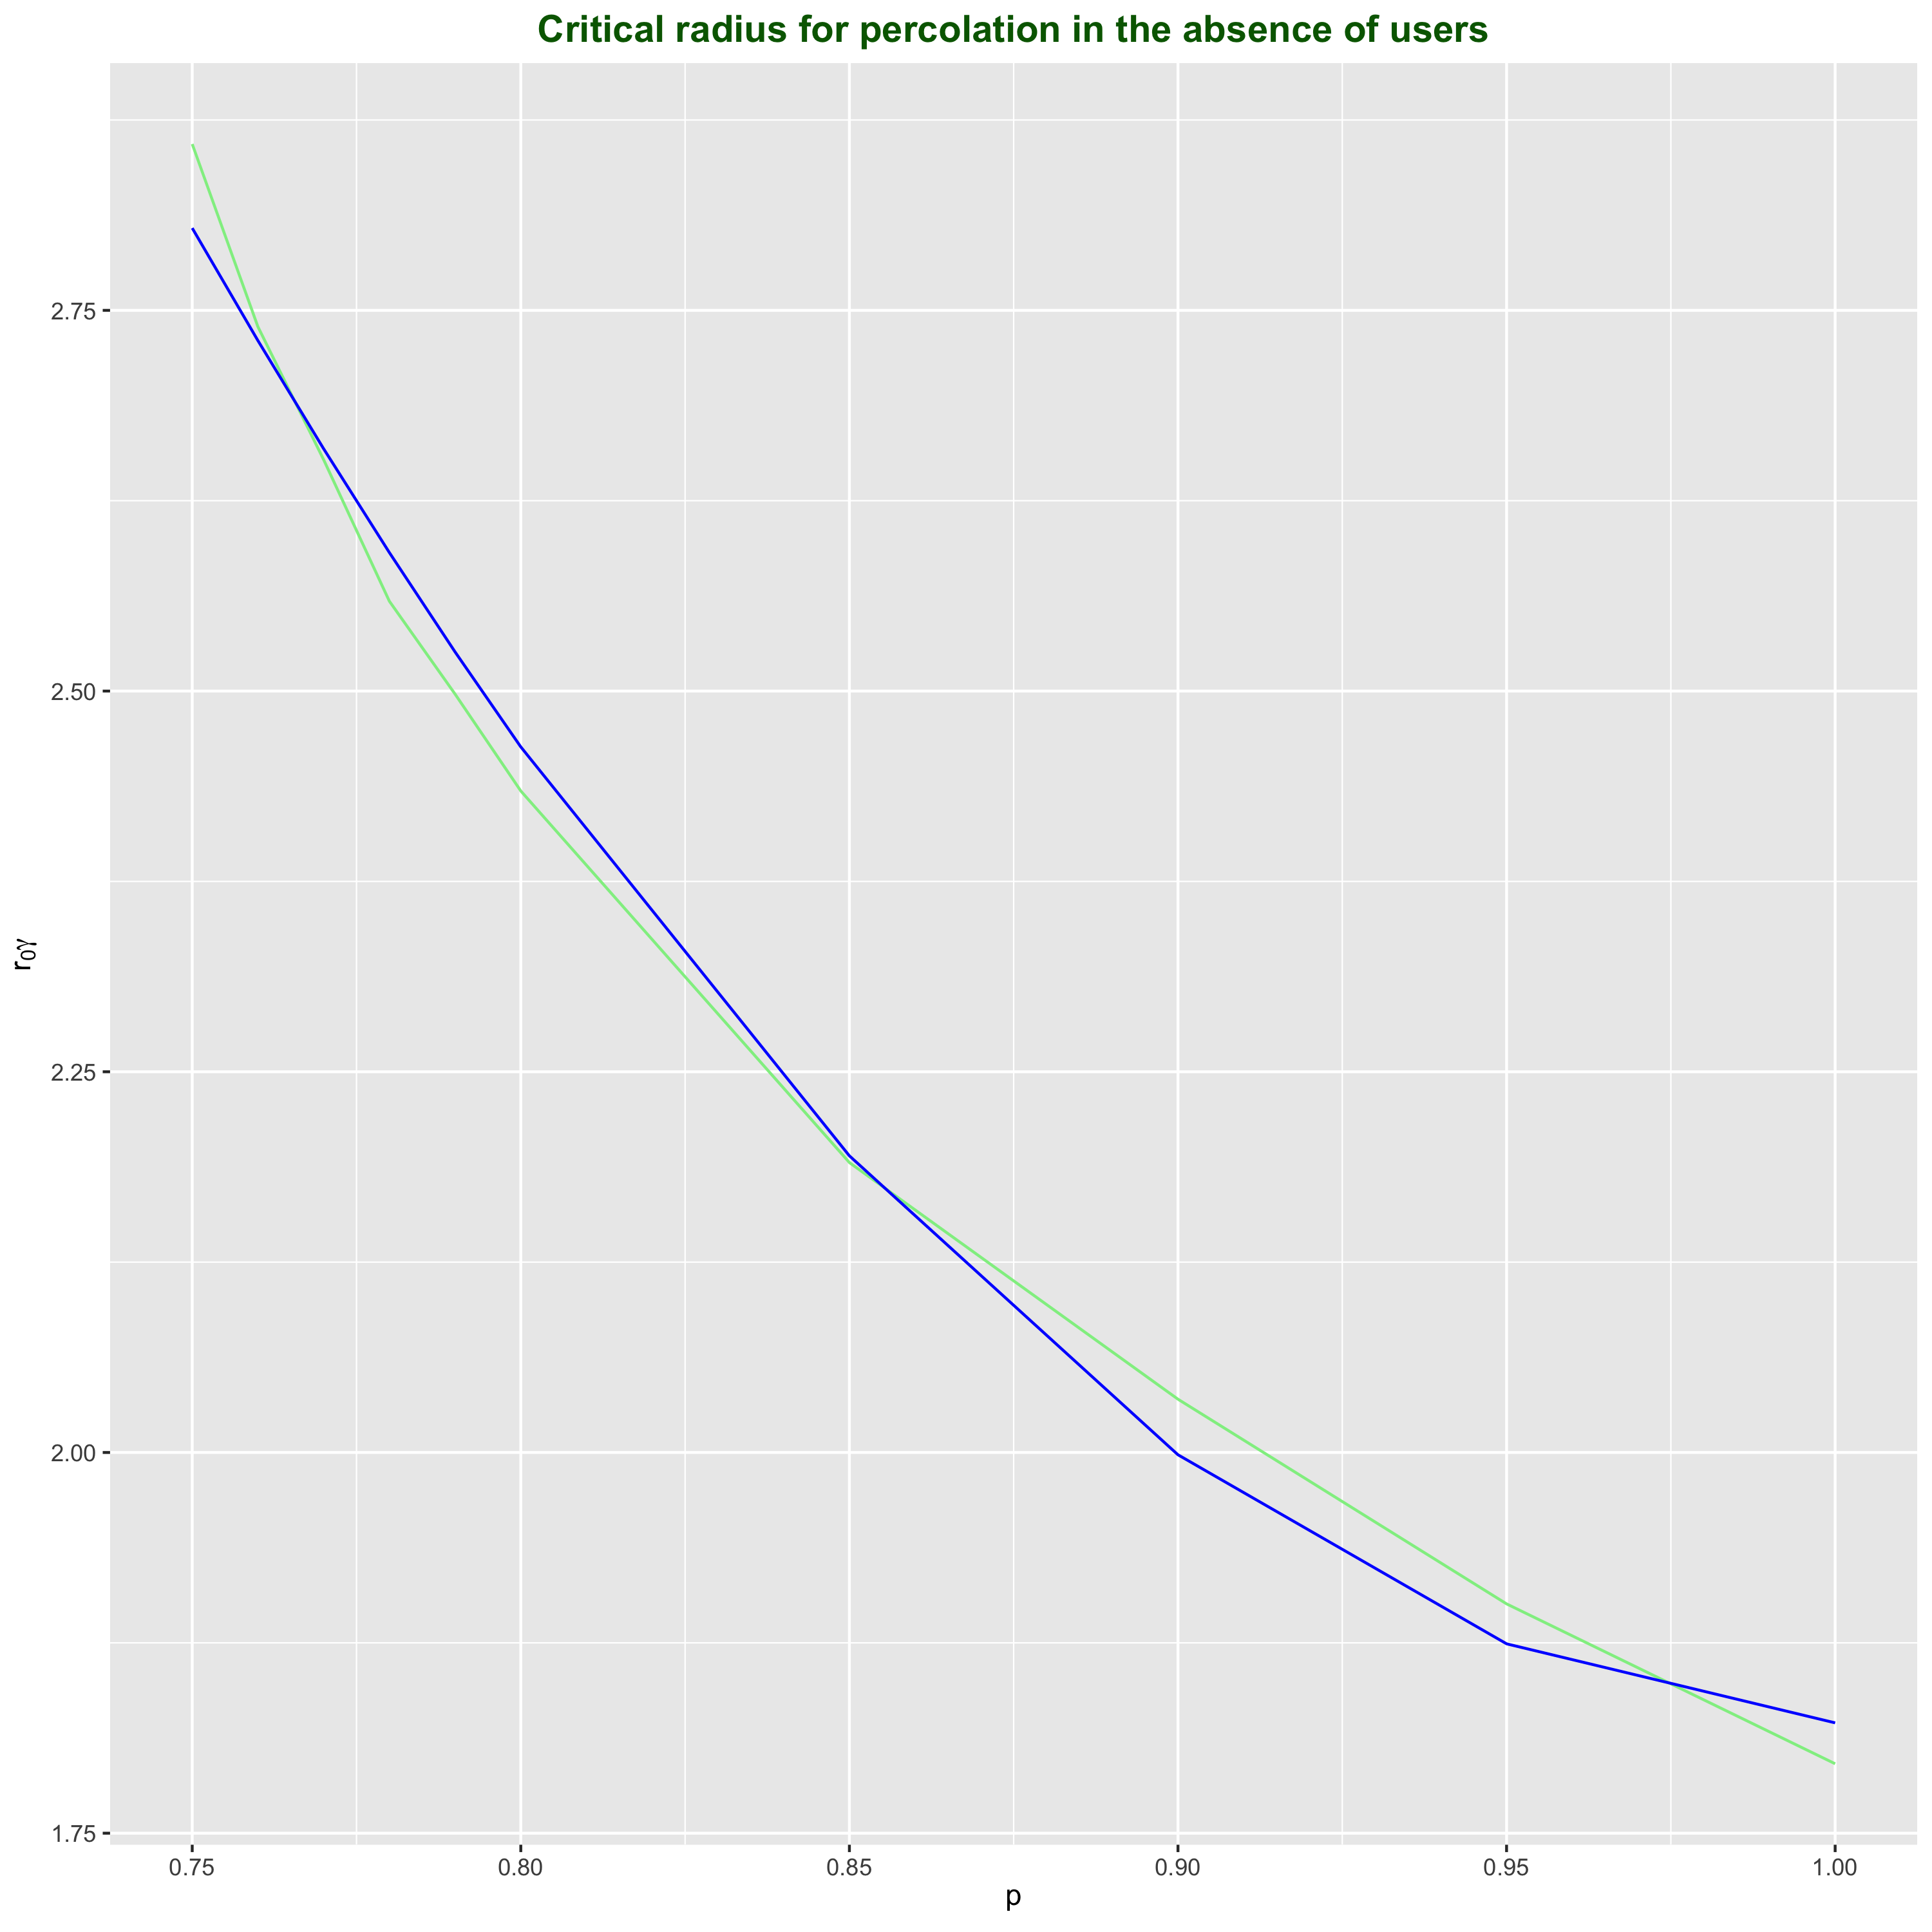
\includegraphics[width=\columnwidth]{Figures/critical-radius-lambda_0-quadratic-fit.png}
\caption{Critical parameter $r_{0}\gamma$ as a function of $p$. The green curve is the simulated curve, the blue one is the quadratic fit.}
\label{quadratic-fit-radius}
\end{figure}
\indent Fig.\ref{quadratic-fit-radius} illustrates the plotting of the critical dimensionless parameter $r_{0}\gamma$ as a function of $p$ for $p \geq 0.75$. We found out that a quadratic model given by \eqref{quadratic-model} yielded a good fit able to explain 91\% of the variance.
\begin{equation}
\label{quadratic-model}
r_{0}\gamma = ap + bp^{2} + c
\end{equation}
The coefficients $a$, $b$ and $c$ can be estimated by linear regression:
\begin{equation}
\begin{array}{l}
a \approx -29.20 \\
b \approx 14.44 \\
c \approx 16.58
\end{array}
\end{equation}
%(Intercept)           p          p2 
   %16.57854   -29.19583    14.43975 
\\
\indent Nevertheless, the D2D communication threshold $r$ is fixed by the technology used and, in practice, remains a parameter on which operators do not have any leverage, unless if they massively invest in research and development. Hence the need for a positive user density so as to try to ensure connectivity of the network. At a short time scale, user density is a physical parameter on which operators could have leverage on, e.g. via commercial means so as to incentivize users to take part in a multihop D2D network.

%change for nicer curves, remove titles? Ask for conventions as what concerns the title, the axes, etc...
%convention : figure comes after the text it is quoted in? %subfigures %position arguments?

\section{Ensuring connectivity by adding users on the streets}
The main question arising from the previous section is about what happens when the D2D technology used is not sufficient to reach the critical radius $r_{0}$ for a given relay proportion $p$. In other words, for $p > p_{c}^{\text{bond,PVT}}$, and $r < r_{0}$, is there a critical user density above which long-range communications are possible?\\
Denote the critical user density by:
\begin{equation}
%same question as for r0
\label{critical-lambda}
\lambda_{c} = \lambda_{c}(r,p) \coloneqq \inf \lbrace \lambda \geq 0, \; \mathcal{G}_{r,0,p} \; \text{percolates} \rbrace  
\end{equation}
Theorem \ref{minimality_theorem} implies that whenever $p < p_{c}^{\text{bond,PVT}}$, we have $\lambda_{c}(r,p)= \infty$ for all $r > 0$. Moreover, the numerical results from Section \ref{radius-influence} ensure that for $p \geq 0.75$ and $r > r_{0}(p)$, we have $\lambda_{c}(r,p)=0$. We are therefore interested in the case where $p > p_{c}^{\text{bond,PVT}}$ and $r < r_{0}(p)$. In particular, do we have $0 < \lambda_{c} < \infty$ ? 

\subsection{Non-triviality of the critical user density}
On a theoretical perspective, we were able to prove that under sufficiently general conditions, the critical user density allowing for long-range communications is indeed positive and finite. Our two main results are the following ones:
\\
\begin{theorem}[Positivity of the critical user density]
%Shall I mention again that S is a PVT, hence stabilising and essentially asymptotically connected?
\label{positivity-critical-lambda}
Assume $p > p^{\text{bond,PVT}}_{c}$. Then there exists an absolute constant $r^{*} > 0$ not depending on $p$ such that whenever $r < r^{*}$, $\lambda_{c}(r,p) > 0$. In other words, long-range communications cannot be achieved in the absence of users if the D2D communication threshold is too small. \\
\end{theorem}
\begin{theorem}[Finiteness of the critical user density]
%same here
\label{finiteness-critical-lambda}
Assume $p > p^{\text{bond,PVT}}_{c}$ and $r < r_{0}(p)$. Then there exists an absolute constant  $p^{*} \in \left[p_{c}^{\text{bond,PVT}},1\right)$, possibly different from $p_{c}^{\text{bond,PVT}}$, such that whenever $p > p^{*}$, $\lambda_{c}(r,p) < \infty $. In other words, long-range communications can be achieved under a sufficiently high (but finite!) user density if the relay proportion is large. \\
\end{theorem}
\indent As the goal of this paper is more about giving numerical estimates, rigorous proofs of Theorems \ref{positivity-critical-lambda} and \ref{finiteness-critical-lambda} will be provided in a companion paper to be published in a mathematical journal. We therefore only give rough sketches of the former proofs and omit tedious technical details. Both proofs crucially rely on the fact that the chosen street system $S$ is a PVT and is therefore stabilizing and asymptotically essentially connected, as explained and proven in \cite{hirsch_continuum_2017}. 
%talk about renormalisation arguments here? Moreover, they appeal to so-called renormalisation techniques \cite{blabla}, which consist in introducing on the same underlying geometry that the one we used a discrete percolation problem, easier to solve than a continuous one... 
\\

\begin{IEEEproof}[Sketch of proof of Theorem \ref{positivity-critical-lambda}]
The proof starts with defaulting to the case $p=1$. Indeed, when $p<1$, there will be fewer possible connexions in the network, so there will need to be more users on the streets to ensure connectivity at a large scale. Thus, we have $\forall \, r > 0, \, \lambda_{c}(r,p) \leq \lambda_{c}(r,1)$. Therefore, it suffices to prove that $\lambda_{c}(r,1) > 0$ for $r$ greater than a certain absolute constant $r^{*}$.   \\
\indent Now, the idea behind stabilization is that the configuration of the network environment in a given observation window only depends from a bounded region including the observation window with high probability. In other words, if two observed regions of the network are sufficiently distant, they are independent. This allows to introduce a discretized site percolation process featuring short-range spatial dependencies only. Well-chosen definitions of open and closed sites in the former process allow to ensure that if the discretized process does not percolate, then neither does $\mathcal{G}_{r,\lambda,1}$. Finally tedious technical details based on the use of the domination by product measures theorem \cite{liggett1997domination} allow to conclude that the discretized process does not percolate if $\lambda$ is sufficiently small and $r < r^{*}$ for some absolute constant $r^{*}$ ($r^{*}$ only depends on the edge length distribution of the edges in a PVT). Hence, our original process does not percolate if $\lambda$ is sufficiently small and $r < r^{*}$. Therefore, $\lambda_{c}(r,1) > 0$ whenever $r < r^{*}$, which concludes the proof.
\end{IEEEproof}

\vspace{1\baselineskip}

\begin{IEEEproof}[Sketch of proof of Theorem \ref{finiteness-critical-lambda}]
The techniques used in this proof are similar to the ones used in the proof of Theorem \ref{positivity-critical-lambda}. In this case, we introduce a discrete percolation process chosen so that if the former process percolates, then so does $\mathcal{G}_{r,\lambda,p}$. Crucially relying on the asymptotic essential connectedness \cite{hirsch_continuum_2017} of the PVT street system $S$ and using again the domination by product measures theorem \cite{liggett1997domination} allows to conclude that the discretized percolation process percolates if $\lambda$ and $p$ are sufficiently large. Hence the result.
\end{IEEEproof}

\vspace{1\baselineskip}

Note that, in Theorem \ref{positivity-critical-lambda}, we had to make an additional assumption $r < r^{*}$, i.e. the D2D communication threshold cannot be too large. This is of course realistic on a technical perspective, and logic on a physical perspective: if $r$ is sufficiently large, as seen in Section \ref{radius-influence}, users are not needed anymore to ensure large-scale connectivity of the network in our model. 

\subsection{Numerical estimations of critical user density}
On a more applied note and in the light of the results given by Theorems \ref{positivity-critical-lambda} and \ref{finiteness-critical-lambda}, it also is of great interest, especially for operators willing to study the technical feasibility of a D2D-enabled network, to get numerical estimates of the critical user density values for a range of parameters $r$ and $p$. This is the issue we tackle in this subsection. \\
\indent The simulation method used to estimate the critical user density $\lambda_{c}$ for given $\gamma$,$r$ and $p$ is merely the same as in Sections \ref{relay-influence} and \ref{radius-influence}: for a given set of parameters $(\gamma,r,p)$ and a grid of values for $\lambda$, we simulate a large number of connectivity graphs $\mathcal{G}_{r,\lambda,p}$ and compute the propostion $h(\lambda)$ of simulations where $\mathcal{G}_{r,\lambda,p}$ percolates. Again, a logistic model gives a good fitting of the estimated curve, and we determine $\lambda_{c}$ by noting the abscissa of the inflexion point of the logistic curve. Fig.\ref{critical-user-estimation} illustrates an example for $p=0.9$ and $r\gamma= 0.3$. 
\begin{figure}[t!]
\centering
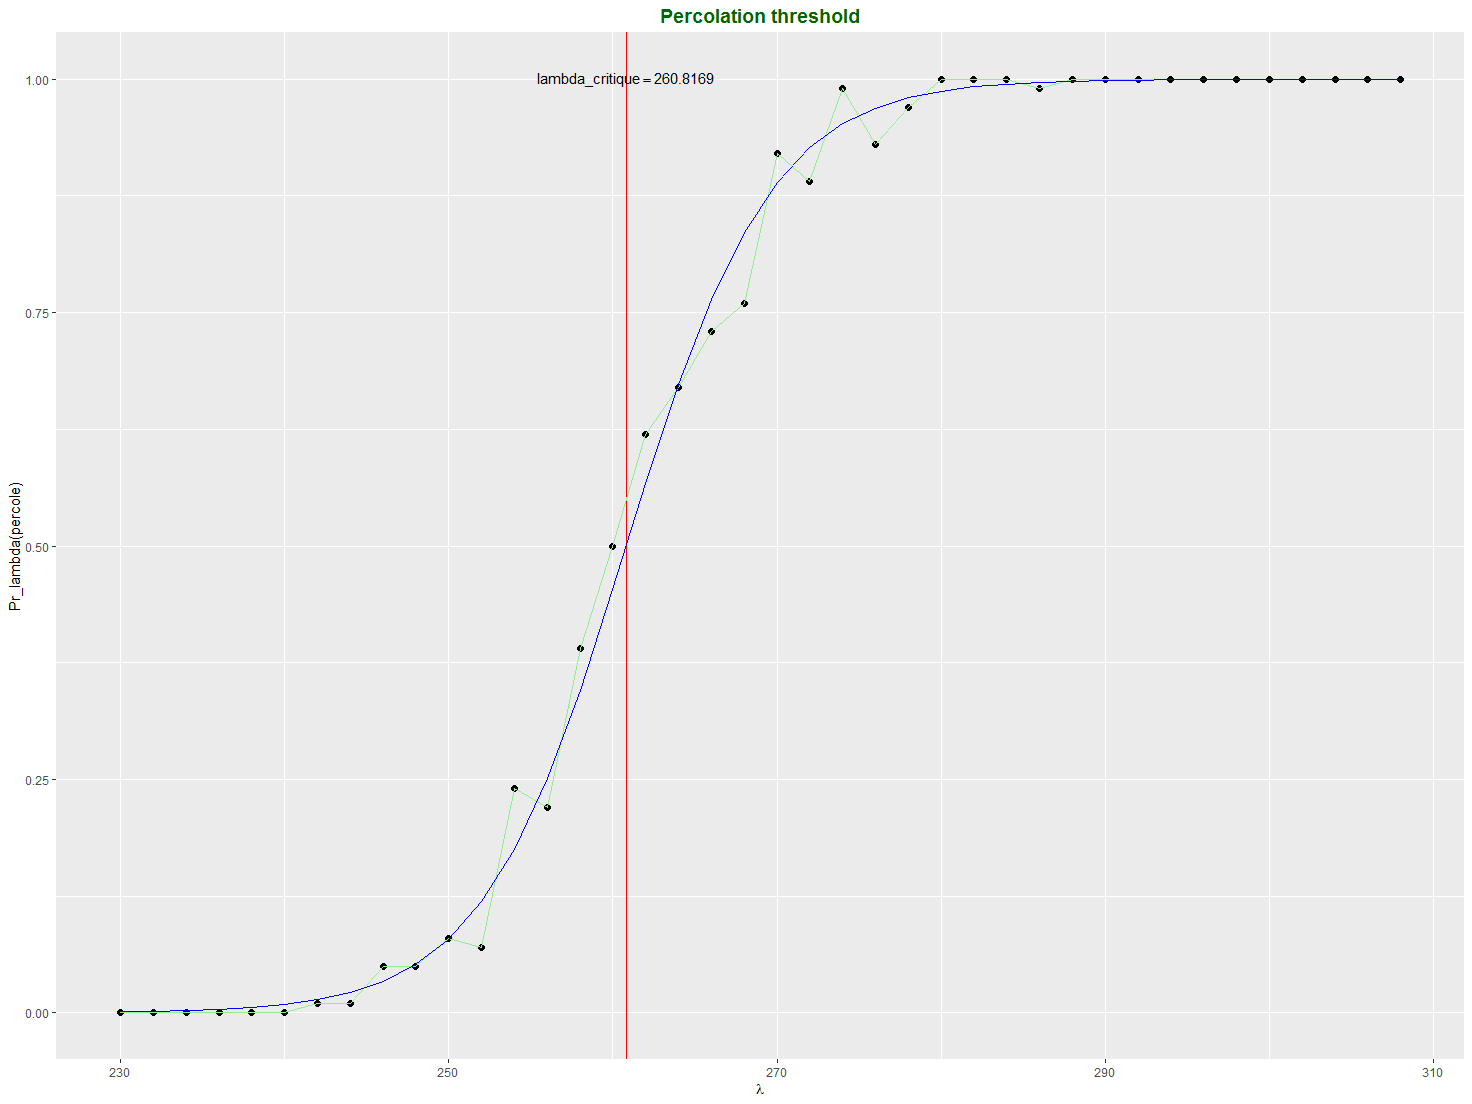
\includegraphics[width=\columnwidth]{Figures/Rplot.png}
\caption{Estimation of $\lambda_{c}$ for $p=0.9$ and $\gamma = 20 \; \text{km/km}^{2}$. The simulation window is of size 10x10 $\text{km}^{2}$ for time-constraint purposes. The green curve is the simulated curve $\lambda \mapsto h(\lambda)$, the blue one is the logistic model and the red vertical line determines the intercept $\lambda_{c}$.}
\label{critical-user-estimation}
\end{figure}
\begin{table}[t!]
\caption{Critical parameter $\lambda_{c}/\gamma$ for a grid of values of $p$ as a function of $r\gamma$. NA stands for Non Applicable data in \cite{cali2018percolation}.} %and comparison with PBM/previous work.
\begin{center}
\begin{tabular}{|c|c|c|c|c|c|c|}
\hline
\multicolumn{7}{|c|}{$\lambda_{c}/\gamma$}\\
\hline
$r\gamma$ & $p=1$ & $p=0.9$ & $p=0.8$ & $p=0.75$ & PBM & NSHOW \cite{cali2018percolation} \\
\hline
0.3 & 12.17 & 13.04 &   & & 15.95 & 11.9 \\
0.5 & 5.304  & 6.226 & & & 5.74 & 5.58 \\
1 & 1.364 & 1.814 & & & 1.435 & NA \\
1.5 & 0.307  & 0.574 & &  & 0.638 & 0.75  \\
2.0 & 0  & 0.023 & & & 0.358  & NA \\
2.5 & 0  & 0 & & & 0.229 & 0.24 \\
3.5 & 0 & 0 & & & 0.117 & 0.12 \\
\hline
\end{tabular}
\label{tab-critical-lambda}
\end{center}
\end{table}
%I should rather add a curve \lambda / \gamma wrt r\gamma
%Table \ref{tab-critical-lambda} presents numerical results %and compares with reference critical densities for percolation of the Poisson Boolean model \cite{blabla} and for percolation models without shadowing on PVT \cite{blabla} --> Then how do we make the comparison? Values of p? Table \lambda / gamma wrt r\gamma and p? 
As mentioned earlier in Section \ref{assumption}, invariant scale factors of our model are $\lambda / \gamma$ and $r\gamma$, which is why we give our results in Table \ref{tab-critical-lambda} in terms of the former two dimensionless parameters. We also include in Table \ref{tab-critical-lambda} a comparison with the celebrated Poisson Boolean model (PBM) \cite[Table 2]{balister_continuum_2005} and with results from \cite{cali2018percolation}, where the authors simulated a model similar to ours without any shadowing effects (NSHOW), i.e. there are only users on streets distributed according to a Cox process and any two users (being in LOS or in NLOS) with reciprocal Euclidean distance less than $r$ are connected. \\
%Comment about the comparison with NSHOW?
\begin{figure*}[t!]
\centering
\begin{minipage}{0.5\textwidth}
  \centering
  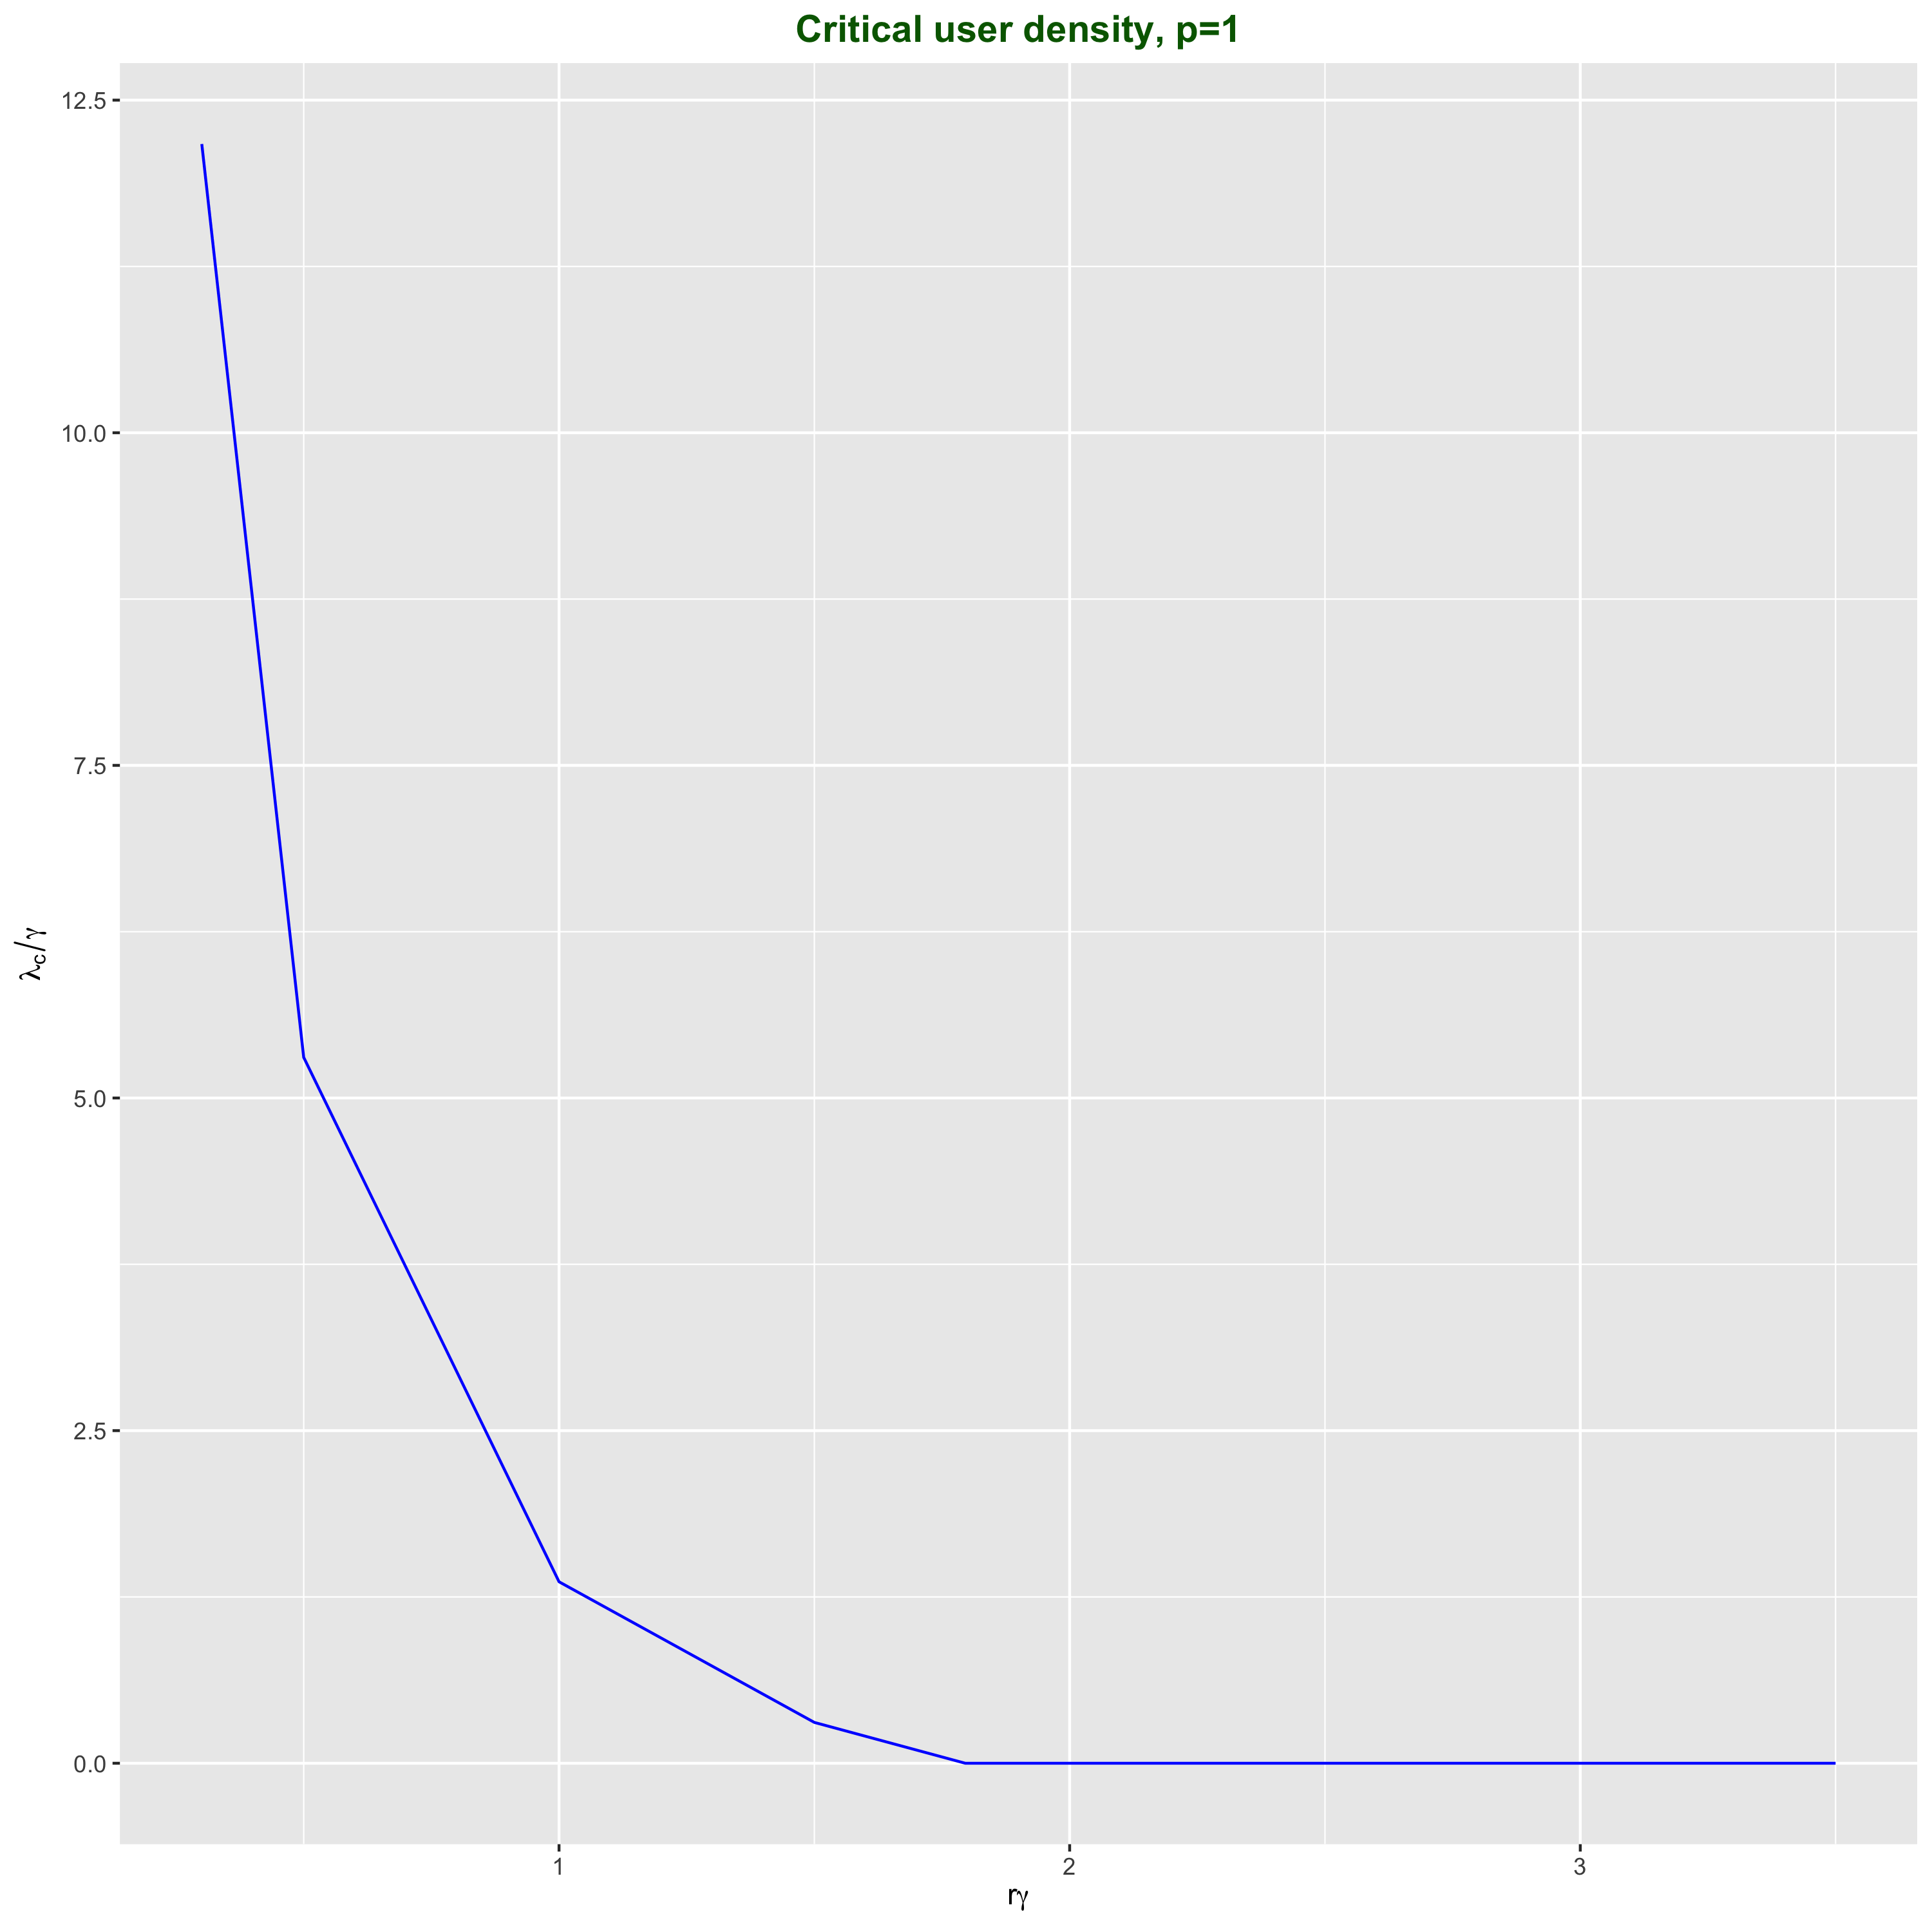
\includegraphics[width=\textwidth]{Figures/critical-lambda-p_1.png}
\end{minipage}%
\begin{minipage}{0.5\textwidth}
  \centering
  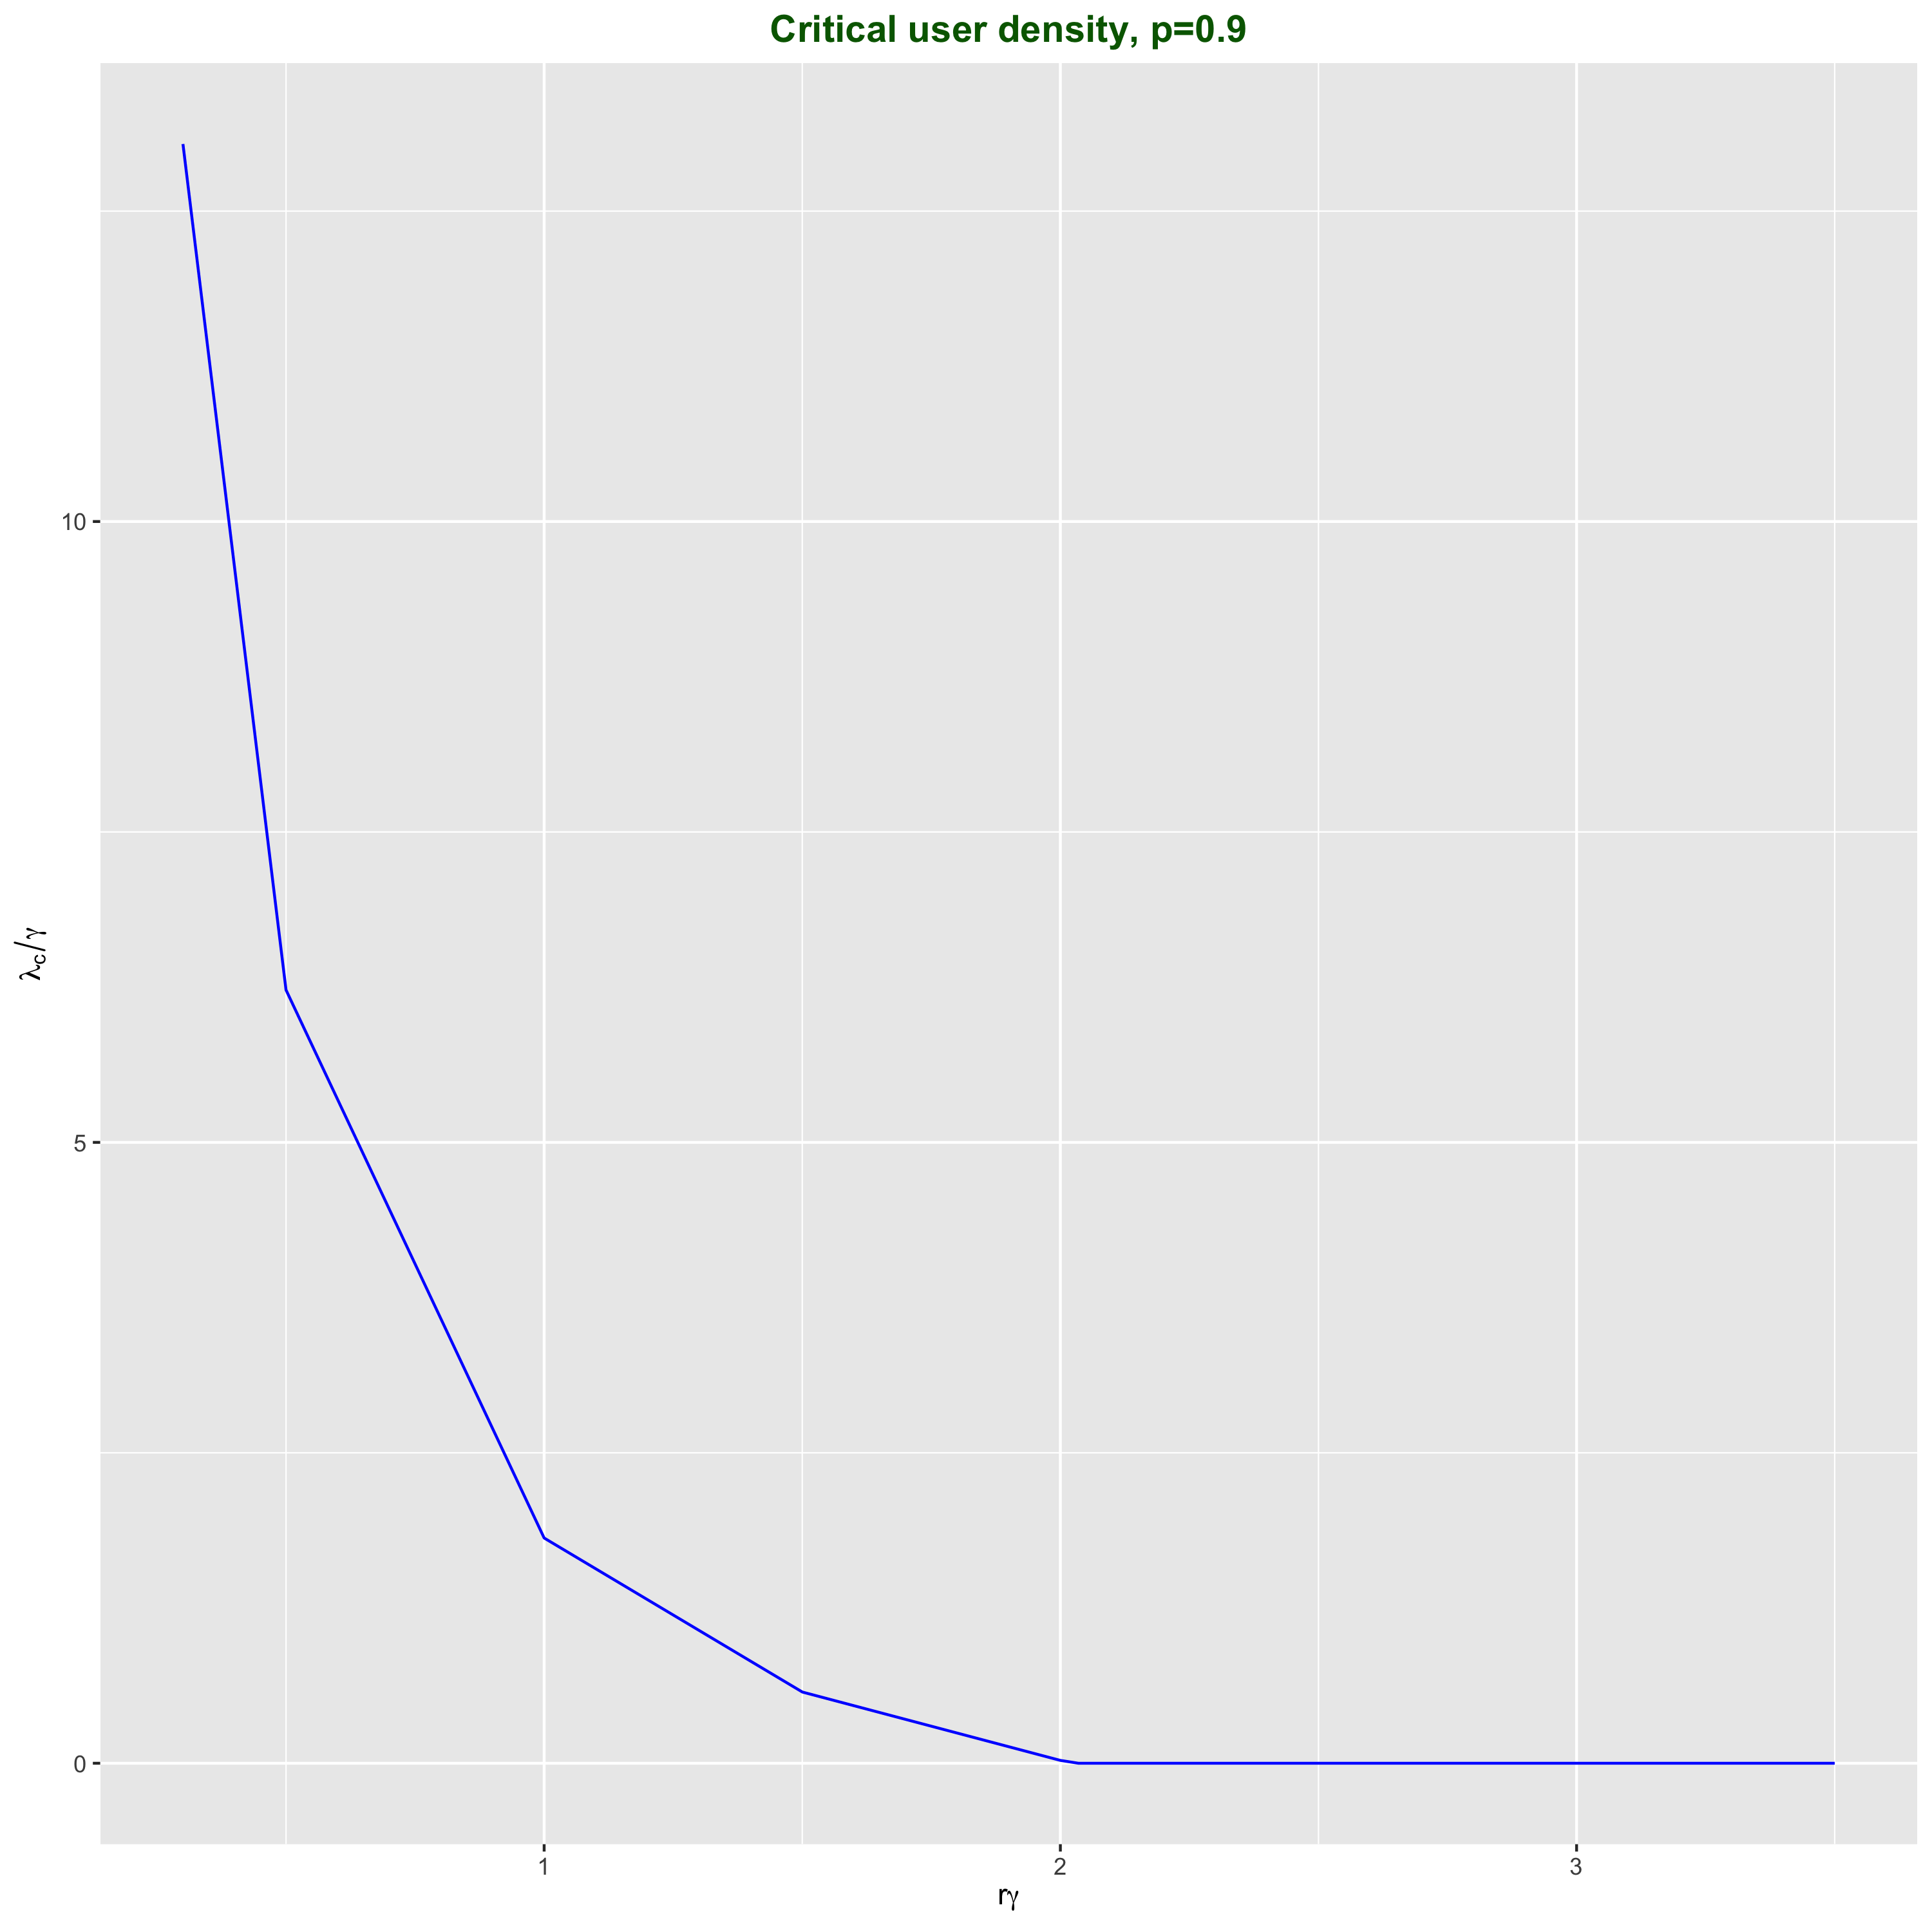
\includegraphics[width=\textwidth]{Figures/critical-lambda-p_0_9.png}
\end{minipage}
\caption{Plotting of the critical dimensionless parameter $\lambda_{c}/ \gamma$ as a function of $r\gamma$ for $p=1$ (left subfigure) and $p=0.9$ (right subfigure). \label{critical-density-comparison}}
\end{figure*}
\indent Fig.\ref{critical-density-comparison} shows the variation of $\lambda_{c} / \gamma$ as function of $r\gamma$. It is clear that the critical parameter $\lambda_{c} / \gamma$ decays exponentially fast in $r\gamma$. An approximation by an inhomogeneous Bernoulli bond percolation model presented in \cite{hirsch_continuum_2017} results in the following formula:
\begin{equation}
\frac{\lambda_{c}}{\gamma}\exp(-r\lambda_{c}) = - \log(b_{c}) \; ,
\end{equation}
where $b_{c} = 0.5$ for a PVT street system. This however does not seem to be a reasonable approximation for our model, especially when  the relay proportion $p$ approaches criticality. Instead, we propose another approach and fit the following model with the statistical software R:
\begin{equation}
\log \left(\frac{\lambda_{c}}{\gamma}\right) = a \left(\frac{r}{\gamma}\right) + b \,
\end{equation}
which is indeed equivalent to an exponential decay:
\begin{equation}
\frac{\lambda_{c}}{\gamma} = \exp \left(a\frac{r}{\gamma}+b\right)
\end{equation}
Once again, $a$ and $b$ can be estimated by a linear regression.
\section{Conclusion and perspectives on future work}
This it the conclusion section. It will be typed later.
\section*{Acknowledgments}
The authors would like to acknowledge 


\bibliographystyle{IEEEtran}
\bibliography{IEEEexample}


\end{document}
